\documentclass[10pt]{article}

\usepackage{caption}
\usepackage{subcaption}
\usepackage{graphicx}
\usepackage{multirow}
\usepackage{wrapfig}
\usepackage{enumerate}
% \usepackage[margin=1.1in]{geometry}

\providecommand{\e}[1]{\ensuremath{\times 10^{#1}}}

\begin{document}

\section{Exercise 1}

\begin{figure}[!ht]
	\centering
	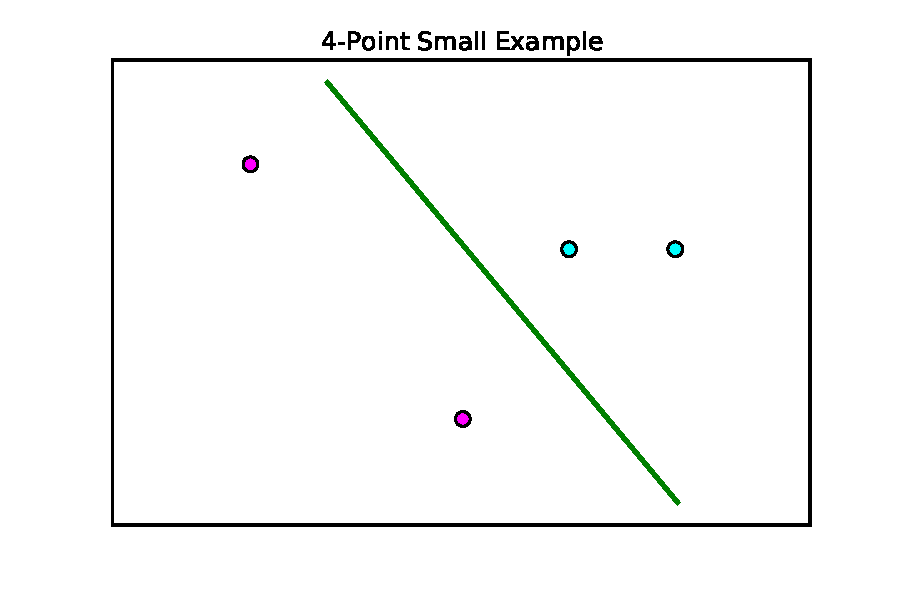
\includegraphics[width=\textwidth]{exercise1-1.pdf}
	\caption{Something}
	\label{fig:1-1}
\end{figure}


1.2 - since smallOverlap was the same, took half the data for test and half for train



2.2: 
* do training set over some values of lambda
* use that to pick lambda
* test on `validation' data and report an error value

2.3:
will need to plot lambda versus sparsity

2.4:
* do training set over some values of bandwidth with lambda = 0
* do validation set over some values of lambda
* test on test and report results

2.5:
* will need to think about this a little bit more.

3.1:
* https://piazza.com/class/hzdfawvtilo7hf?cid=434
* L2 regularization, linear case
* http://blog.datumbox.com/machine-learning-tutorial-the-multinomial-logistic-regression-softmax-regression/

* maybe need to save coefficients or predictions or something?

3.1 - LR:
* 2 features, 100 pts, 2 classes, l = 0.01 -> error = .485
* might need to randomly select subsets of data points

* tips for getting numerics to work better:
	* normalize data beforehand (then don't forget to re-normalize later)
	* 

3.2 - multiclass SVM:
* used http://scikit-learn.org/stable/modules/generated/sklearn.svm.LinearSVC.html
* can do this SO FAST it doesn't even make sense to try to do this by myself.
* tried an array of l values with L1 loss (multiclasssvm.py), best L with random partitioning of data into 3 sets. rigorous stopping criteria
* hinge loss, l2 regularization: 
	* validation error: .187
	* test error: .261
	* l: 0.01
* squared loss, l1 regularization:
	* validation error: .143
	* test error: .143
	* l: 7e-7

\end{document}